


\section{Experiments}
\label{sec:experiments}
\Copy{sow}{
In this section, we explore the techniques via binary classification problems on an artificial dataset (i.e., Moon) and 41 real-world datasets i.e., Knowledge Extraction based on Evolutionary Learning (KEEL), University of California Irvine (UCI), Credit Card Fraud, with a diversity of imbalance ratios and different numbers of features. Samples in Moon have two features, while other datasets contain various numbers of features and imbalance ratios.} Dataset details are described in Table \ref{tab:dataDecription}.  
The implementation steps to balance datasets follow Algorithm \ref{alg:SIMPOR}. To evaluate our proposed balancing technique, we compare the classification performance to different widely-used and state-of-the-art techniques. More specifically, We compare \Methodname{} to SMOTE \cite{chawla_smote:_2002}, Borderline-SMOTE \cite{bordersmote},  ADASYN \cite{ADASYN}, DeepSMOTE \cite{deepsmote}, Gaussian Distribution Based Oversampling (GDO) \cite{bib:GDO}, SVMCS \cite{cssvm}, EE \cite{EE}. To evaluate the classifications performance for skewed datasets, we measure widely-used metrics, i.e., F1-score and Area Under The Curve (AUC). 



\subsection{Implementation Detail}
This section describes the general settings and implementation details for the experimental techniques. Our implementation code is publicly available on Github \footnote{\url{https://github.com/nsh135/_SIMPOR_}}.  


\subsubsection{\Methodname{} settings}

In order to find the informative subset, we leverage entropy-based active learning. We first utilize a neural network model playing a role as a classifier to find high-entropy samples (Note that the classifier for finding the informative subset differs from the classifiers for the final classification evaluation after all balancing techniques are applied to the data). The detailed steps are introduced in Section \ref{sec:EAL}. The model contains two fully connected hidden layers with \textit{relu} activation functions and 10 neurons in each layer. The output layer applies the soft-max activation function. The model is trained in a maximum of 300 epochs with an early stop option when the loss is not significantly improved after updating weights. The model is trained firstly on a random set of three samples each class (six samples two classes). This model is then used to estimate entropy scores for the remaining data. We then select next 20  highest entropy samples ($k$=20) for the next informative data batch. This batch is concatenated to the initial batch for updating the classifiers and accumulated to the informative set. The steps are repeated until the informative set reaches desire informative portion (IP). In these experiments, we set IP=0.3 corresponding to 30 percent of the training size selected for the informative set. 


To solve the optimization problem in Equation \ref{prob:optimazation} for finding optima (this differs from the classification optimization for the evaluation) introduced in Section \ref{sec:solvingOptimization}, we use a gradient ascent method with the gradient rate of $1e-5$ and the maximum iteration of 300.   

\subsubsection{Evaluation Classification settings}
Considering each imbalanced dataset as a classification problem, we use the classification testing performance for the technique comparison. Each dataset is randomly split into two parts, 80\% for training and 20\% for testing. The classifiers are trained on training sets after applying the techniques. The results are reported on the raw testing sets (There isn't any technique applied on the testing sets; thus, they are also possibly class imbalanced). We use F1-score and AUC for the evaluation metrics as they are suitable and widely used to evaluate imbalanced data. Reported testing results for each dataset are the averages of 5 experimental trials.

The classifiers are constructed by neural networks with the input and output sizes corresponding to the number of datasets' features and unique labels. We use the same classifier structure (number of hidden layers, number of neurons in each layer, learning rate, optimizer) for all compared datasets. The detail of neural network implementation is described in Table \ref{tab:model_setting}. 
For baseline technique settings, we follow the experimental parameter sets in \cite{bib:GDO} as we share very similar datasets and comparison techniques. For DeepSMOTE settings, the DCGAN input and output sizes are modified to adapt with each dataset, while other settings is taken from the initial parameter set in \cite{deepsmote}.


\begin{table}[htbp!]
	\centering
	\caption{Classification models' setting for each dataset.}
	%\rule{\linewidth}{3cm}
	\label{tab:model_setting}
	\resizebox{0.9\columnwidth}{!}{%
	
\begin{tabular}{lp{29.57em}}
	\toprule
	Method & \multicolumn{1}{l}{Parameter} \\
	\midrule
	SIMPOR & \multicolumn{1}{l}{k\_neighbors=5, r\_distribtuion=Gaussian, IP=0.3} \\
	GDO   & \multicolumn{1}{l}{k\_neighbors=5, d=1} \\
	SMOTE & \multicolumn{1}{l}{k\_neighbors=5, sampling\_strategy=`auto',random\_state=None} \\
	BL-SMOTE & \multicolumn{1}{l}{k\_neighbors=5, sampling\_strategy=`auto', random\_state=None} \\
	ADASYN & \multicolumn{1}{l}{k\_neighbors=5, sampling\_strategy=`auto', random\_state=None} \\
	EE    & \multicolumn{1}{l}{\#estimators=10, Estimater=AdaBoostClassifier} \\
	DeepSMOTE   & \multicolumn{1}{l}{Sigma=1, Lambda=0.1} \\
	\midrule
	Classifier & \multicolumn{1}{l}{Parameter} \\
	\midrule
	Architecture & \multicolumn{1}{l}{neuron/layer=100, \#layers=3} \\
	Optimization & optimizer=`adam',  epochs=200, batch\_size=32, learning\_rate=0.1, reduce\_lr\_loss(factor=0.9,epsilon=1e-4,patience=5) \\
	\bottomrule
\end{tabular}%

	}
\end{table}%


\subsection{\Methodname{} on artificial Moon dataset}

\begin{figure}[h!]	
	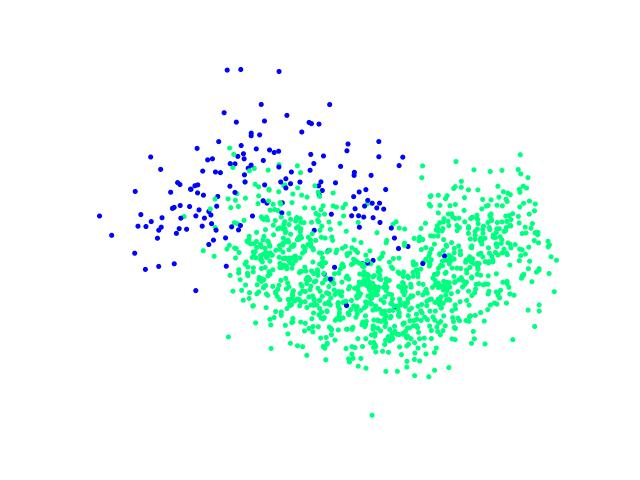
\includegraphics[width=0.9\linewidth]{Figures/moon/ImbalancedData}
	\caption{Artificial class imbalanced Moon dataset with IR of 7:1.}
	\label{fig:raw_moon}
\end{figure}


\begin{figure*}[th]
	\centering
	%[trim=left bottom right top, clip]
	\begin{subfigure}[]{0.3\linewidth}
		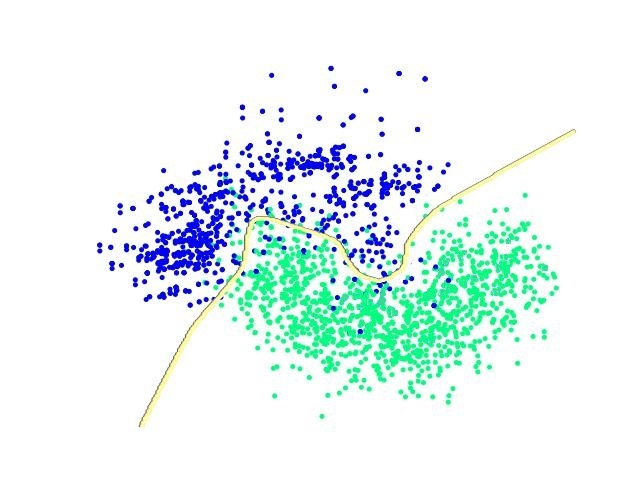
\includegraphics[width=\linewidth]{Figures/moon/Training_Data_PLot_SIMPOR}
		\caption{\Methodname{}.}
		\label{fig:simpor_moon}
	\end{subfigure}
	\hspace{0.1em}% 
	\begin{subfigure}[]{0.3\linewidth}
		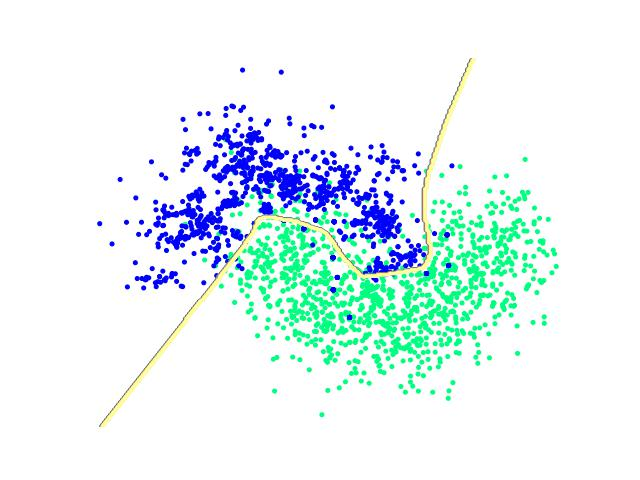
\includegraphics[width=\linewidth]{Figures/moon/Training_Data_PLot_GDO}
		\caption{GDO.}
		\label{fig:gdo_moon}
	\end{subfigure}
	\hspace{0.1em}% 
	\begin{subfigure}[]{0.3\linewidth}
		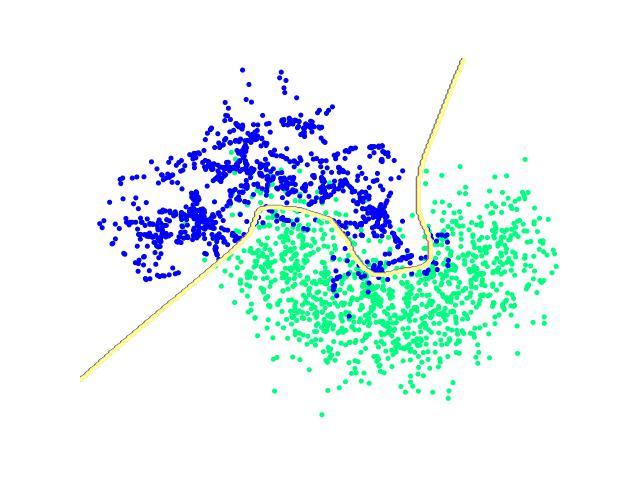
\includegraphics[width=\linewidth]{Figures/moon/Training_Data_PLot_SMOTE}
		\caption{SMOTE.}
		\label{fig:smote_moon}
	\end{subfigure}
	\\
	\begin{subfigure}[]{0.3\linewidth}
		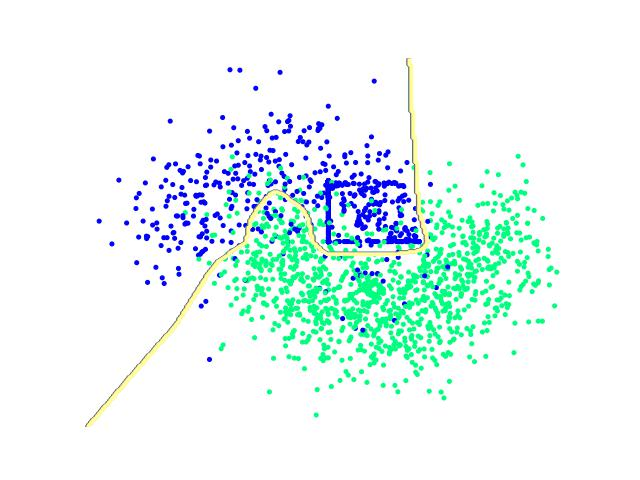
\includegraphics[width=\linewidth]{Figures/moon/Training_Data_PLot_DeepSMOTE}
		\caption{ DeepSMOTE.}
		\label{fig:deepsmote_moon}
	\end{subfigure}
	\hspace{0.1em}% 
	\begin{subfigure}[]{0.3\linewidth}
		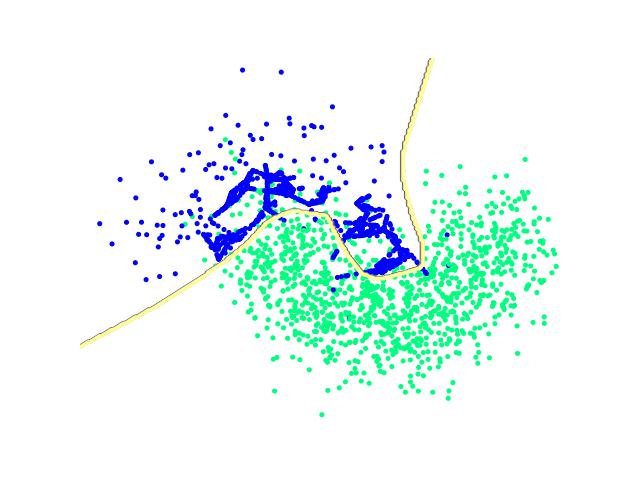
\includegraphics[width=\linewidth]{Figures/moon/Training_Data_PLot_BorderlineSMOTE}
		\caption{BorderlineSMOTE.}
		\label{fig:border_smote_moon}
	\end{subfigure}
	\hspace{0.1em}% 
	\begin{subfigure}[]{0.3\linewidth}
		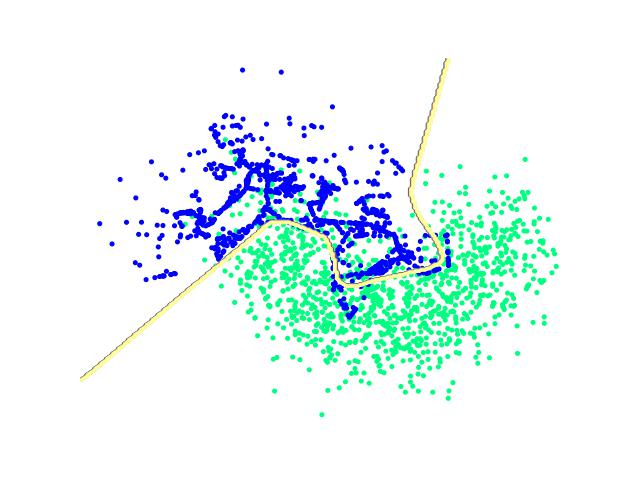
\includegraphics[width=\linewidth]{Figures/moon/Training_Data_PLot_ADASYN}
		\caption{ADASYN. }
		\label{fig:adasyn_moon}
	\end{subfigure}
	
	\caption{Data plot and model's decision boundary visualization for Moon Dataset over different techniques.}
	\label{fig:MoonResults}
\end{figure*}

\Copy{moonGeneration}{
We implement techniques on an artificial 2-dimension dataset for demonstration purposes. We first generate the balanced synthetic MOON dataset using python library \textit{sklearn.datasets.make\_moons}. The generated MOON contains 3000 samples labeled in two classes, and each instance has two numerical features with values ranging from 0 to 1. We then make the dataset artificially imbalanced with an Imbalance Ratio of 7:1 by randomly removing 1285 samples from one class.} As a result, the training dataset becomes imbalanced, as visualized in Figure \ref{fig:raw_moon}.

Figure \ref{fig:MoonResults} captures the classification for different techniques. We also visualize the model decision boundaries to provide additional information on how the classification models are affected. We use a fully connected neural network described in Table \ref{tab:model_setting} to classify the data.




% Table generated by Excel2LaTeX from sheet 'Accuracy'
\begin{table}[htbp!]
	\centering
	\caption{Classification Result on Moon Dataset.}
	\resizebox{\columnwidth}{!}{%
		
	\begin{tabular}{crcccccc}
		Metric &       & SIMPOR & SMOTE & BL-SMOTE & DeepSMOTE   & ADASYN & GDO \bigstrut[b]\\
		\hline
		F1-score &       & 0.883 & 0.824 & 0.827 & 0.842 & 0.785 & 0.817 \bigstrut[t]\\
		AUC   &       & 0.961 & 0.957 & 0.955 & 0.959 & 0.955 & 0.959 \\
	\end{tabular}%

}
	\label{tab:MoonPerformance}
\end{table}%

\subsubsection{Results and Discussion}
From the visualization shown in Figure \ref{fig:MoonResults} and the classification performance results in Table \ref{tab:MoonPerformance}, it is clear that \Methodname{} performs better than others by up to 10\% on F1-score and 1.1\% on AUC. We can see that DeepSMOTE (DeepSM) creates dense squared noise and pushes the decision boundary to the majority class. Due to the fact that SMOTE-based methods does not take the informative region into account, unbalanced data in this area lead to a severe error in decision boundary. In Figures \ref{fig:adasyn_moon} and \ref{fig:border_smote_moon}, BorderlineSMOTE (BL-SMOTE) and ADASYN focus on the area near the model's decision boundary, but they inherit a drawback from SMOTE; any noise or mislabeled samples can, unfortunately, create very dense bridges crossing the expected border and lead to decision errors. Figure \ref{fig:gdo_moon} shows that GDO also generates local gaussian groups of samples near the boder and thus create errors. This phenomenon might cause by a few mis-labeled sample points. In contrast, by generating neighbors of minority samples in the direction towards the minority class and balancing the informative region, \Methodname{} (Figure \ref{fig:simpor_moon}) helps the classifier to make a better decision with a solid smooth decision boundary. Poorly-placed synthetic samples are significantly less than that of others. 


\subsection{\Methodname{} on forty-one real datasets}
\label{subsec:41Datasets}
\Copy{datasetDetail}{
In this section, we compare the proposed technique on 41 real two-class datasets with a variable number of features and Imbalance Ratios, i.e., KEEL datasets \cite{ KEEL_detail,KEEL_dataset}, UCI datasets fetched from Sklearn tool \cite{imbalancedlearnFetch_datasetsx2014, uci_imbalance_dataset} and Credit Card Fraud \cite{kaggleCreditCard} dataset. Since the original Credit Card Fraud contains a large number of banking normal and fraud transaction samples (284,807) which significantly reduces our experimental efficiency, we reduced the dataset size by randomly removing normal class transactions to reach an imbalance ratio of 3.0. Other datasets are kept as their original versions after removing bad samples (containing Null values). The datasets are described in Table \ref{tab:dataDecription}. 
}
\subsubsection{Classification results}
\label{sec:classificationResult}
% Table generated by Excel2LaTeX from sheet 'MacroF1'




\begin{figure}[h!]
	\centering
	%[trim=left bottom right top, clip]
	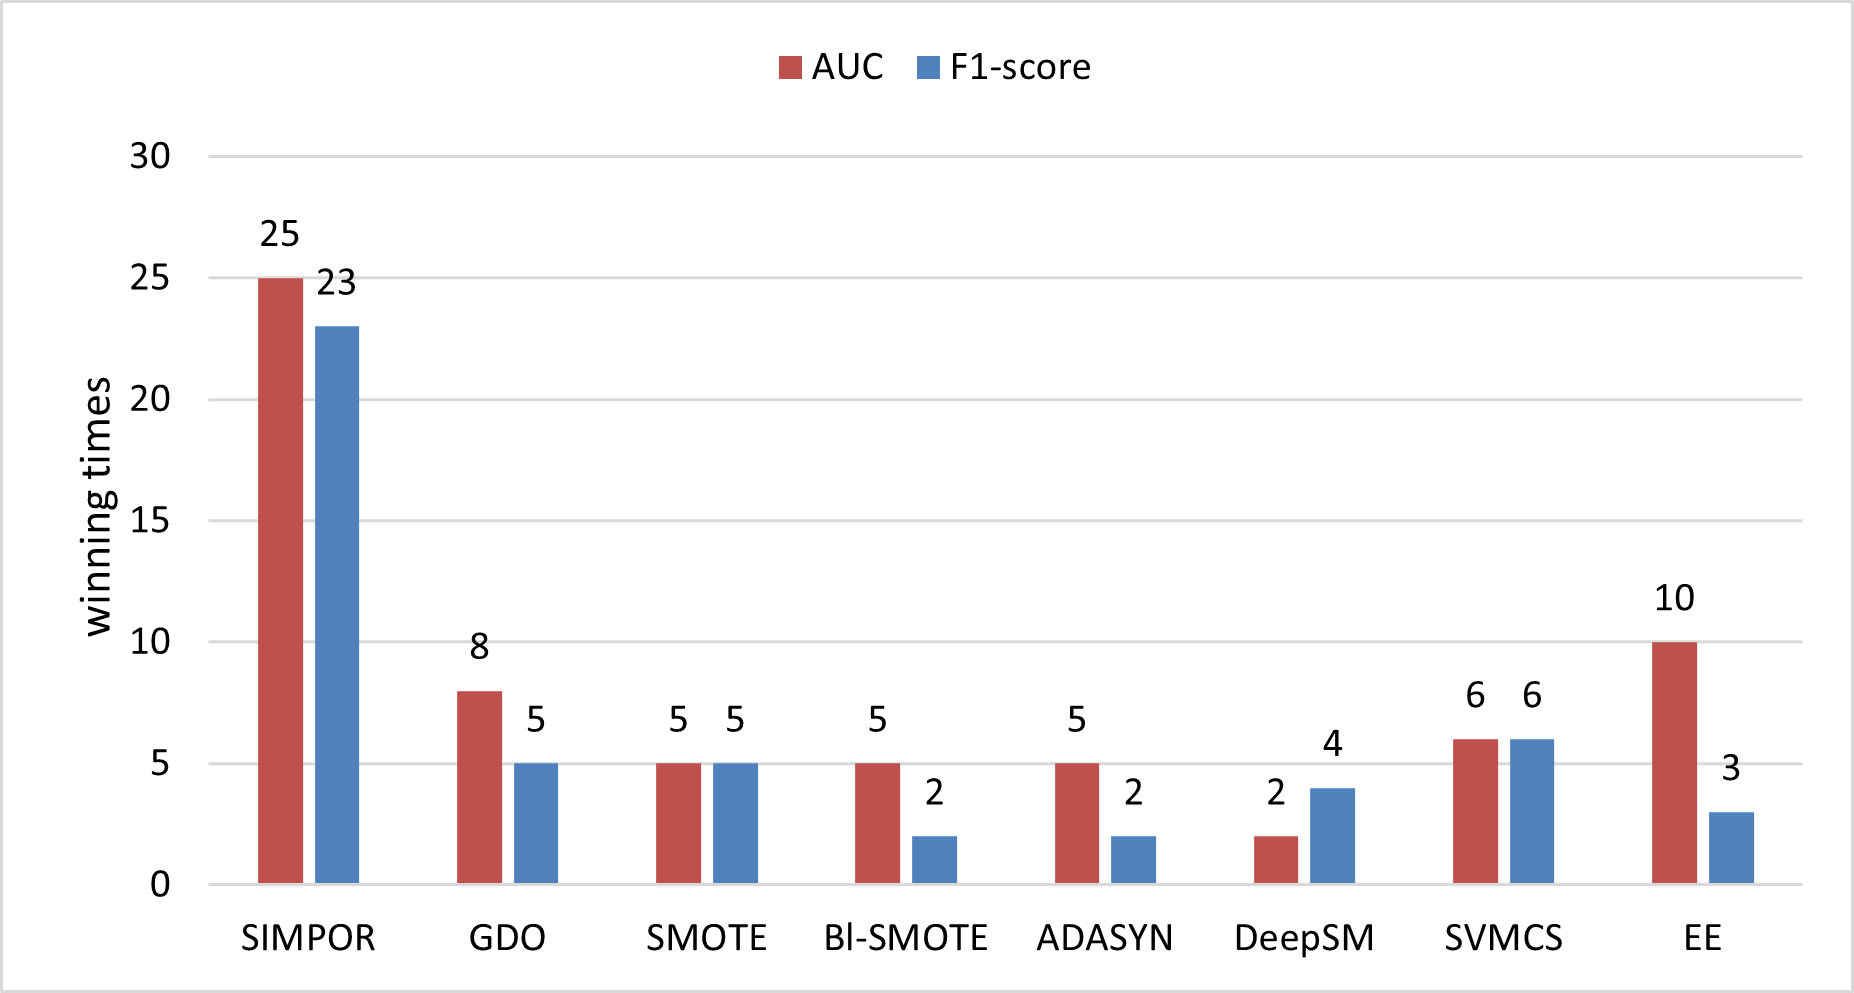
\includegraphics[width=\linewidth ]{Figures/winning_times}
	\caption{Winning times over 41 datasets.}
	\label{fig:winingTimes}
\end{figure}

Table \ref{tab:F1AllDatasets}, \ref{tab:AUCAllDatasets}, \ref{tab:Precision} and \ref{tab:Recall} show the classification F1-score, AUC, Precision, and Recall results, respectively. The highest scores for each dataset are highlighted in bold style. 
\Copy{winningTime}{We also provide the summary of the F1 and AUC scores by ``winning times" scores. We count the number of datasets for which a technique achieves the highest scores among the compared techniques and name this number ``winning times". For convention, if more than two techniques share the same highest score, the winning times will be increased for each technique. Figure \ref{fig:winingTimes} shows a summary of winning times.} 

As we can see from the table, the proposed technique outperforms others on both evaluation metrics, F1-score and AUC. More specifically, \Methodname{} hits 23 F1-score winning times and 25 AUC winning times. Its number of F1-score winning times at 23 four times better than the second winner (SVMCS) at 6, and its AUC winning times at 25 doubles the second AUC winners (EE) at 10. 


\subsection{Statistical Test.}
	\label{sec:wilcoxon}

To further evaluate the effectiveness of the technique, we also performed a Wilcoxon Signed Rank Test \cite{wilcoxon} on the 41 dataset results (F1 score and AUC). Wilcoxon hypothesis test is relevant to our study as it is a non-parametric statistical test and does not require a specific distribution assumption for the results. On the other hand, 41 data points (corresponding to 41 datasets results) are sufficient to support this test. Our null hypothesis is that the difference between the proposed technique results and those of the other technique is insignificant. Wilcoxon signed-rank test outputs are computed over the 41 dataset results and return a p-value for each technique pair. We then compare the p-value with the significant value $\alpha = 0.05$. Suppose the p-value is smaller than $\alpha$. In that case, the evidence is sufficient to reject the hypothesis, which means the proposed technique does make a significant difference from the others, and vice versa. Table \ref{tab:wilcoxonTest} shows the Wilcoxon p-value results.

	\begin{table}[htbp]
		\centering
		\caption{Wilcoxon Signed Rank Hypothesis Test results.}
		
		\begin{tabular}{lcc}
			\toprule
			& \multicolumn{2}{c}{p-value} \\
			\midrule
			SIMPOR vs. & \multicolumn{1}{l|}{F1-score} & \multicolumn{1}{l}{AUC} \\
			\midrule
			GDO   & 1.82E-03 & 1.93E-03 \\
			SMOTE & 2.66E-03 & 6.64E-05 \\
			BL\_SMOTE & 4.22E-03 & 1.63E-04 \\
			ADASYN & 2.89E-03 & 6.13E-04 \\
			DeepSM   & 6.40E-04 & 2.57E-04 \\
			SVMCS & 2.74E-03 & 3.40E-02 \\
			EE    & 1.99E-03 & 2.17E-02 \\
			\bottomrule
		\end{tabular}%
		\label{tab:wilcoxonTest}%
	\end{table}%

As we can see from Table \ref{tab:wilcoxonTest}, the p-values are all smaller than the critical value of 0.05. Thus, the null hypothesis can be rejected as the supporting evidence is sufficient. In other words, the statistical result shows that the proposed technique makes a significant improvement compared to others.     



\subsection{Processing Time.}
\label{sec:processingTime}
Data processing times for oversampling-based approaches on 41 datasets are compared to provide a more comprehensive comparison. We don't compare them to the other approaches, i.e., cost-sensitive learning and ensemble learning, because they only need negligible data processing time as they focus on classifiers other than improving the data. The processing time was recorded from our machine, which uses an Intel i7 32-thread processor and two NVIDIA 3090 Ti GPUs. 
Table \ref{tab:ProcessingTime} shows the recorded processing time over 41 datasets. Overall, our technique takes longer than others as we have to compute the kernel estimation for each data point, as mentioned in Section \ref{sec:implementation}. Similarly, DeepSMOTE generally suffers high time consuming cost because it heavily relies on underlying heuristic methods. In other words, the proposed technique is slower, but it provides better F1 and AUC scores than others.

\begin{table}[htbp]
	\centering
	\caption{Processing time (in seconds) over 41 datasets.}
	\resizebox{0.97\columnwidth}{!}{%
		
		\begin{tabular}{lcccccc}
			\toprule
			& SIMPOR & GDO   & SMOTE & BL-SMOTE & ADASYN & DeepSM \\
			\midrule
			glass1 & 0.1147 & 0.0576 & 0.0020 & 0.0033 & 0.0032 & 0.8587 \\
			wisconsin & 2.0805 & 0.1769 & 0.0024 & 0.0044 & 0.0046 & 1.2004 \\
			pima  & 0.2032 & 0.2066 & 0.0025 & 0.0049 & 0.0050 & 1.2297 \\
			glass0 & 0.2157 & 0.0553 & 0.0023 & 0.0035 & 0.0036 & 0.8601 \\
			yeast1 & 0.2457 & 0.4749 & 0.0035 & 0.0108 & 0.0104 & 1.4846 \\
			haberman & 0.0517 & 0.1560 & 0.0022 & 0.0033 & 0.0036 & 0.9246 \\
			vehicle1 & 0.4365 & 0.1237 & 0.0025 & 0.0059 & 0.0059 & 1.4147 \\
			vehicle2 & 6.2913 & 0.1512 & 0.0029 & 0.0053 & 0.0061 & 1.3976 \\
			vehicle3 & 0.2821 & 0.1237 & 0.0024 & 0.0060 & 0.0061 & 1.3487 \\
			creditcard & 2.1200 & 0.3783 & 0.0087 & 0.0184 & 0.0182 & 1.7980 \\
			glass-0-1-2-3\_vs\_4-5-6 & 0.3376 & 0.0459 & 0.0023 & 0.0035 & 0.0035 & 0.8407 \\
			vehicle0 & 7.3645 & 0.1198 & 0.0024 & 0.0054 & 0.0058 & 1.2953 \\
			ecoli1 & 0.0418 & 0.0337 & 0.0010 & 0.0018 & 0.0017 & 0.9310 \\
			new-thyroid1 & 0.5352 & 0.0304 & 0.0015 & 0.0024 & 0.0024 & 0.8590 \\
			new-thyroid2 & 0.3881 & 0.0359 & 0.0025 & 0.0033 & 0.0031 & 0.8747 \\
			ecoli2 & 0.2516 & 0.0266 & 0.0011 & 0.0017 & 0.0016 & 0.9733 \\
			glass6 & 0.3196 & 0.0268 & 0.0014 & 0.0025 & 0.0023 & 1.0744 \\
			yeast3 & 0.1374 & 0.2422 & 0.0023 & 0.0060 & 0.0059 & 1.6699 \\
			ecoli3 & 0.0658 & 0.0378 & 0.0015 & 0.0025 & 0.0024 & 0.9647 \\
			page-blocks0 & 7.9654 & 2.0918 & 0.0045 & 0.0143 & 0.0138 & 3.6029 \\
			yeast-2\_vs\_4 & 2.4310 & 0.0624 & 0.0017 & 0.0028 & 0.0028 & 1.0286 \\
			yeast-0-5-6-7-9\_vs\_4 & 0.0868 & 0.0632 & 0.0016 & 0.0029 & 0.0027 & 0.9809 \\
			vowel0 & 4.7675 & 0.1312 & 0.0018 & 0.0039 & 0.0037 & 1.2410 \\
			glass-0-1-6\_vs\_2 & 0.0482 & 0.0207 & 0.0013 & 0.0023 & 0.0022 & 0.9133 \\
			glass2 & 0.0501 & 0.0227 & 0.0013 & 0.0024 & 0.0024 & 0.8855 \\
			yeast-1\_vs\_7 & 0.4697 & 0.0420 & 0.0017 & 0.0026 & 0.0026 & 1.0355 \\
			glass4 & 0.1141 & 0.0197 & 0.0012 & 0.0024 & 0.0023 & 0.9469 \\
			ecoli4 & 0.1087 & 0.0310 & 0.0015 & 0.0024 & 0.0024 & 0.9393 \\
			page-blocks-1-3\_vs\_4 & 1.8742 & 0.0445 & 0.0015 & 0.0027 & 0.0026 & 0.9992 \\
			abalone9-18 & 2.9722 & 0.0716 & 0.0015 & 0.0028 & 0.0026 & 1.2095 \\
			yeast-1-4-5-8\_vs\_7 & 0.0881 & 0.0673 & 0.0017 & 0.0031 & 0.0028 & 1.0803 \\
			glass5 & 0.2815 & 0.0241 & 0.0017 & 0.0033 & 0.0036 & 0.8550 \\
			yeast-2\_vs\_8 & 0.1239 & 0.0441 & 0.0016 & 0.0027 & 0.0028 & 0.9849 \\
			car\_eval\_4 & 0.4381 & 0.1746 & 0.0026 & 0.0066 & 0.0049 & 1.6616 \\
			wine\_quality & 0.1622 & 0.8587 & 0.0030 & 0.0144 & 0.0137 & 3.3128 \\
			yeast\_me2 & 0.1060 & 0.1379 & 0.0018 & 0.0042 & 0.0039 & 1.7350 \\
			yeast4 & 0.1083 & 0.1386 & 0.0018 & 0.0041 & 0.0039 & 1.6314 \\
			yeast-1-2-8-9\_vs\_7 & 0.0924 & 0.0757 & 0.0017 & 0.0031 & 0.0030 & 1.3069 \\
			yeast5 & 0.1188 & 0.1312 & 0.0019 & 0.0037 & 0.0040 & 1.6181 \\
			yeast6 & 0.0613 & 0.1419 & 0.0018 & 0.0037 & 0.0036 & 1.6382 \\
			abalone19 & 0.0890 & 0.3161 & 0.0022 & 0.0053 & 0.0054 & 3.0168 \\
			\bottomrule
		\end{tabular}%
		
	}
	\label{tab:ProcessingTime}%
\end{table}%






